% !TeX root = vampy.tex
%vampy-ug.tex
% user guides for VAMPy (image analysis part of VAMP project)

\section{User Guide}\label{userguide}

\emph{Being in active development, the state of the program might be quite different from what is written here!}

As it is now (not packaged in self-contained executable) you need the following software to be installed on your computer to run VAMPy:
\begin{itemize}
	\item Python 2.7.2 (\url{http://www.python.org}
	\item NumPy 1.6.1 (\url{http://www.scipy.org}
	\item SciPy 0.9 (\url{http://www.scipy.org}
	\item matplotlib 1.0.1 (\url{http://matplotlib.sourceforge.net/})
	\item wxPython 2.8.12.1 (\url{http://www.wxpython.org}
	\item Python Image Library 1.1.7 (\url{www.pythonware.com/products/pil/}) 
\end{itemize}
All of the above is Open Source and freely available from respective websites. Version numbers are the ones with which the software was developed and tested, but it might also work with older versions and hopefully will work with future versions of Python language and packages. The program is cross-platform, it runs on Windows (tested), Linux/Unix (tested) and Mac (not tested) as long as all dependencies are met.

\subsection{What you can do with it}\label{vampy-features}
\emph{Warning: list of features is actively changed!}

Currently you can:
\begin{itemize}
	\item Open images of aspirated pipette and view them as stack of images.
	\item Crop the unnecessary parts of the image, rotate it as needed and save this settings for future reuse.
	\item Load corresponding pressure file or read pressures from image filenames.
	\item Analyze the geometry of the image and obtain plots for total area of the vesicle, its volume etc.
	\item Check suspicious points by analyzing single images to see whether the image analysis succeeded.
	\item Obtain the plot of tension vs dilation and corresponding value for the bending rigidity or stretching elasticity from fitting of data.
	\item Export results of geometry analysis and tensions calculations to ASCII file.
	\item Load manually measured geometry data and applied pressure from text files, calculate corresponding dilations and tensions and fit them for getting bending rigidity and stretching elasticity.
	\item As the above but load already manually calculated tensions and dilations from text file.
\end{itemize}

\subsection{User Interface}\label{vampy-ui}
\begin{itemize}
	\item Main window (figure \ref{fig:vampymain})
		\begin{figure}[htbp]
			\centering
			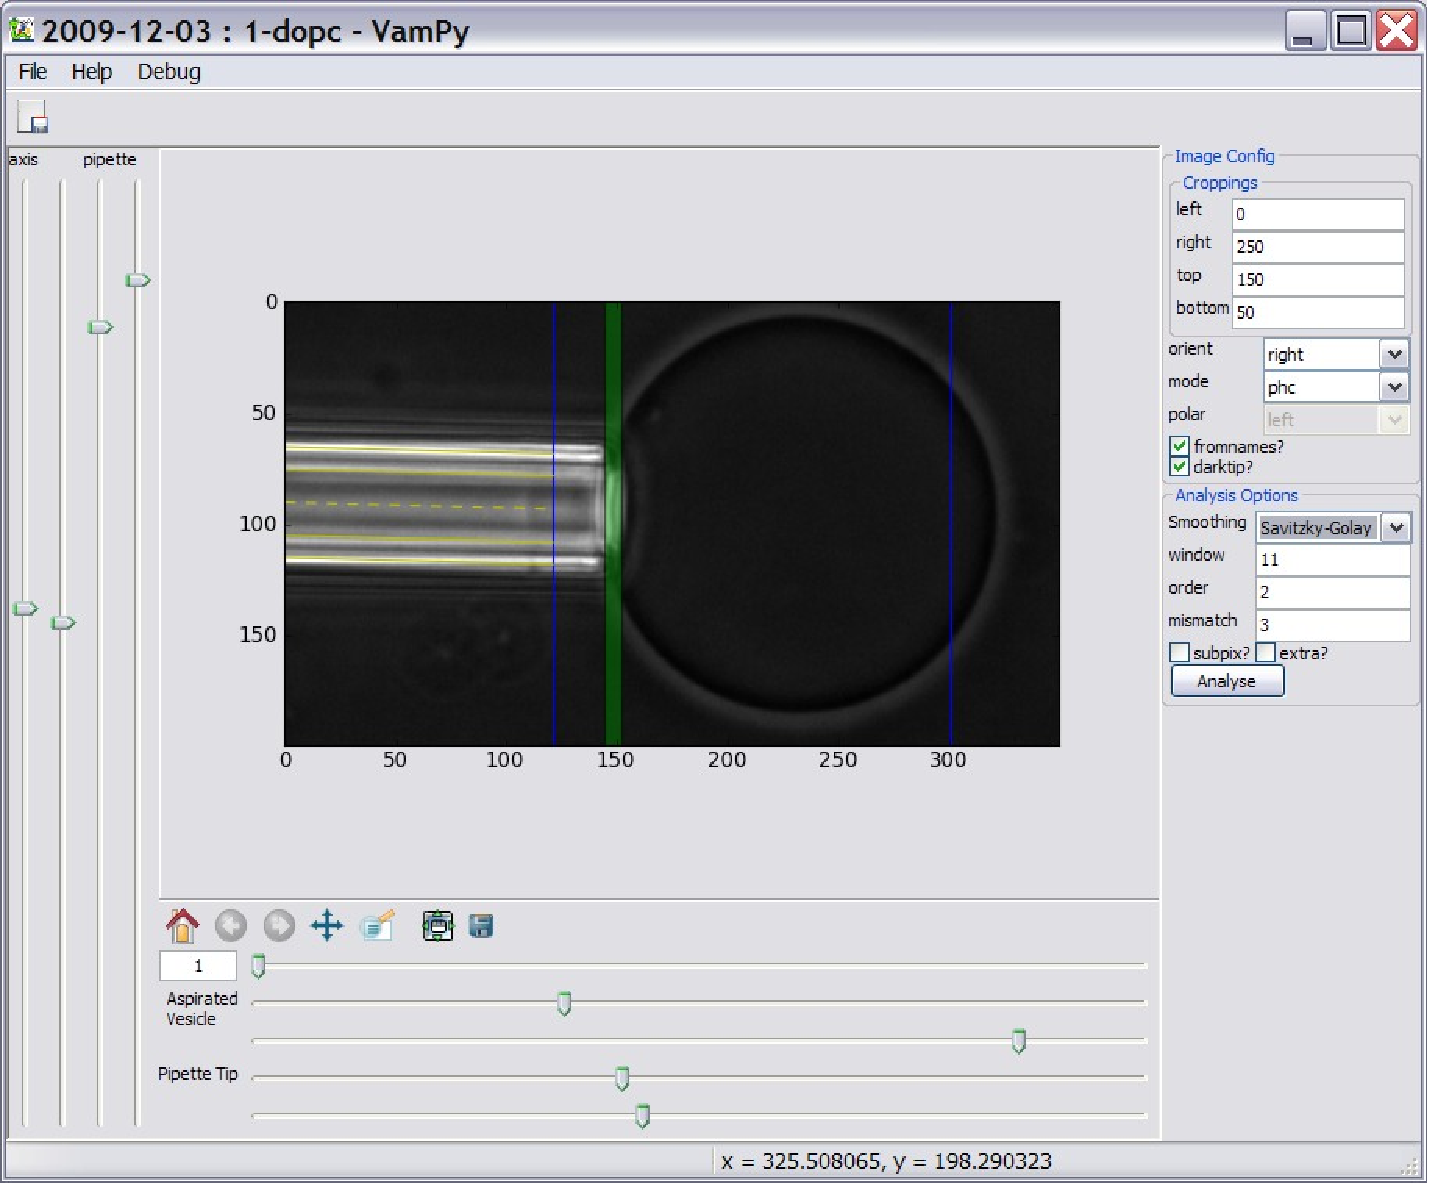
\includegraphics[width=1.00\textwidth]{figs/vampymain.pdf}
			\caption{VAMPy main window}
			\label{fig:vampymain}
		\end{figure}
		\begin{enumerate}
				\item Menu Bar - quite self-explanatory
					\begin{itemize}
						\item File - open directory, exit application
						\item Help - About info, Help (not implemened yet, shows the same info as ``About''
						\item Debug - Debug single image (for analysing image recognition performance), reload (for developers - reloads math modules without restarting GUI)
					\end{itemize}
				\item Tool Bar - contains buttons for some actions (``Open images folder'' and ``Save image config'')
				\item Image panel:
					\begin{enumerate}
						\item Image with region lines and pipette lines
						\item Image toolbar (zoom, pan, adjust subplots, go back and forward between views, save plot as image - does not affect analysis, only representation)
						\item Image slider - scrolls through the images
						\item Region sliders - control region lines for aspirated tip, outer vesicle and pipete mouth
						\item Axis sliders - control the estimation of the pipette axis position
						\item Pipette sliders - control the estimation (radius and walls thickness) of pipette position
					\end{enumerate}
				\item Image Config panel
					\begin{enumerate}
						\item Croppings - used to crop the image
						\item Orientation - for rotation the image
						\item Mode - type of the image (phase contrast or dic)
						\item Polar - type of the dic image
						\item fromnames - how to load pressures, from images filenames (checked) or from pressure file (unchecked)
						\item darktip - what to count for pipette mouth, brightest(unchecked) or the darkest (checked) pixels
					\end{enumerate}
				\item Analsis Options panel
					\begin{enumerate}
						\item Smoothing -- type of applied smoothing (Savitzky-Golay or Gauss readily available)
						\item window - full window size for the smoothing filter (odd integer since point plus same number of points to the left and to the right)
						\item order - used for smoothing the image while processing (polinomial order for Savitzky-Golay, blurring strength for Gauss)
						\item mismatch - the maximal difference between pixel and subpixel resolution to tolerate subpixel routine as successful \emph{(not implemented yet, ignored)}
						\item extra - output extra information as NumPy saved arrays (NPZ) and python pickles \emph{(not implemented yet, ignored)}
						\item subpixel - use subpixel resolution \emph{(not implemented yet, ignored)}
						\item Analyse - start processing 
					\end{enumerate}
				\item Status Bar - when the cursor is in the image/plot shows current coordinates 
		\end{enumerate}
	\item Geometry window (figure \ref{fig:vampygeom})
		\begin{figure}[htbp]
			\centering
			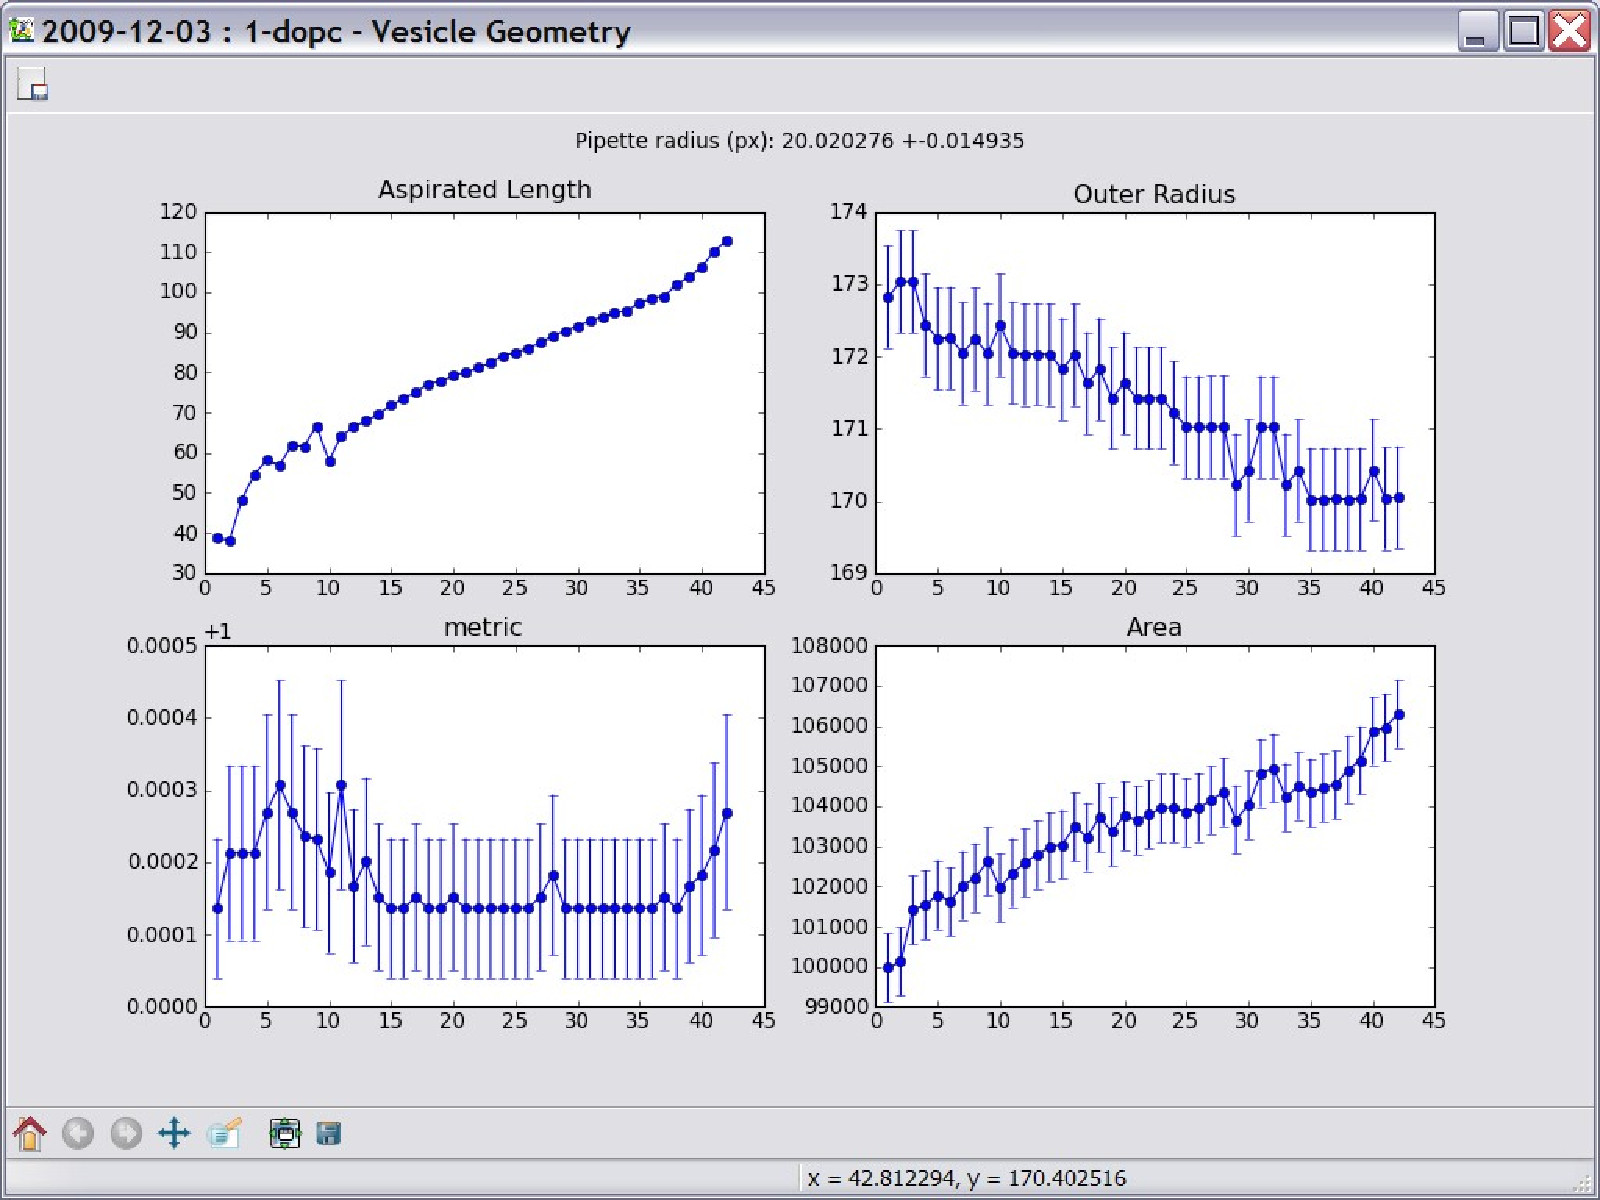
\includegraphics[width=1.00\textwidth]{figs/vampygeom.pdf}
			\caption{VAMPy vesicle geometry window}
			\label{fig:vampygeom}
		\end{figure}
		\begin{enumerate}
			\item Toolbar - buttons to open external geometry file and to save all the calculated data to the ASCII file
			\item Plots - plots of various calculated parameters - currently aspirated length, outer vesicle radius, vesicle total volume and metric (related to the tilt of the axis with 1 being perfectly horizontal). Calculated pipette inner radius is also displayed.
			\item image toolbar - the same as on main window
			\item status bar - the same as on main window
		\end{enumerate}
	\item Fitting window (figure \ref{fig:vampyfit})
		\begin{figure}[htbp]
			\centering
			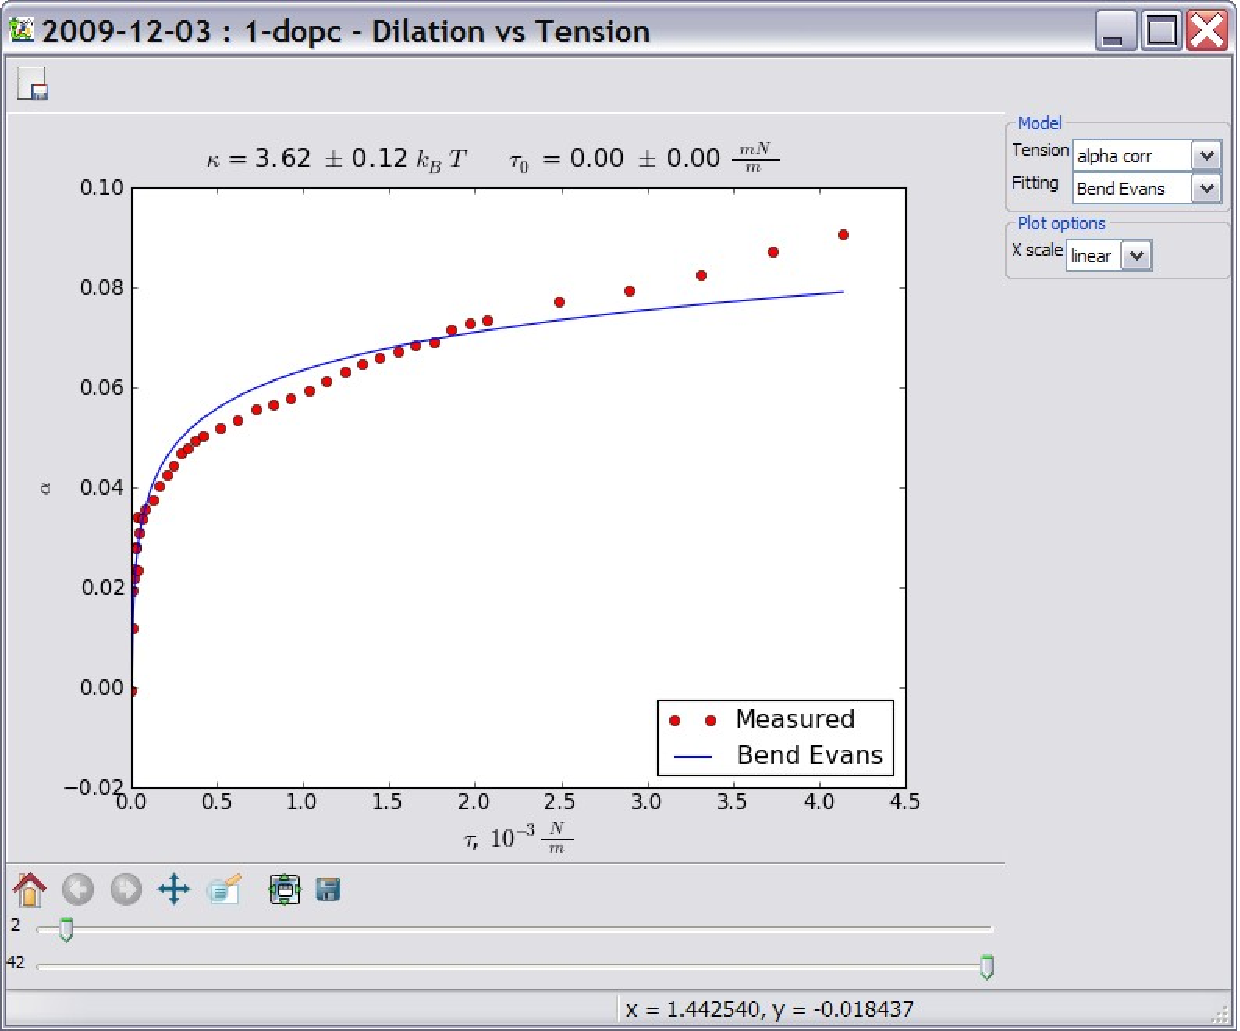
\includegraphics[width=1.00\textwidth]{figs/vampyfit.pdf}
			\caption{VAMPy fitting window}
			\label{fig:vampyfit}
		\end{figure}
		\begin{enumerate}
			\item toolbar - buttons to open external file with tensions/dilations and to save calculated tensions and dilations to ASCII file (for example to analyse/fit it with other tools)
			\item plot of the dilation vs tension - both experimental points and fitted line are shown, with fitted values printed on top
			\item range slider - choose what range of values to fit
			\item Model parameters
				\begin{enumerate}
					\item Tension model used for calculation of tensions/dilations
					\item Model to fit data with
				\end{enumerate}
			\item plot options - currently only choice for x coordinate as linear or log10
			\item image toolbar - the same as on main window
			\item status bar - the same as on main window
		\end{enumerate}
	\item Debug window (figure \ref{fig:vampydebug})
		\begin{figure}[htbp]
			\centering
			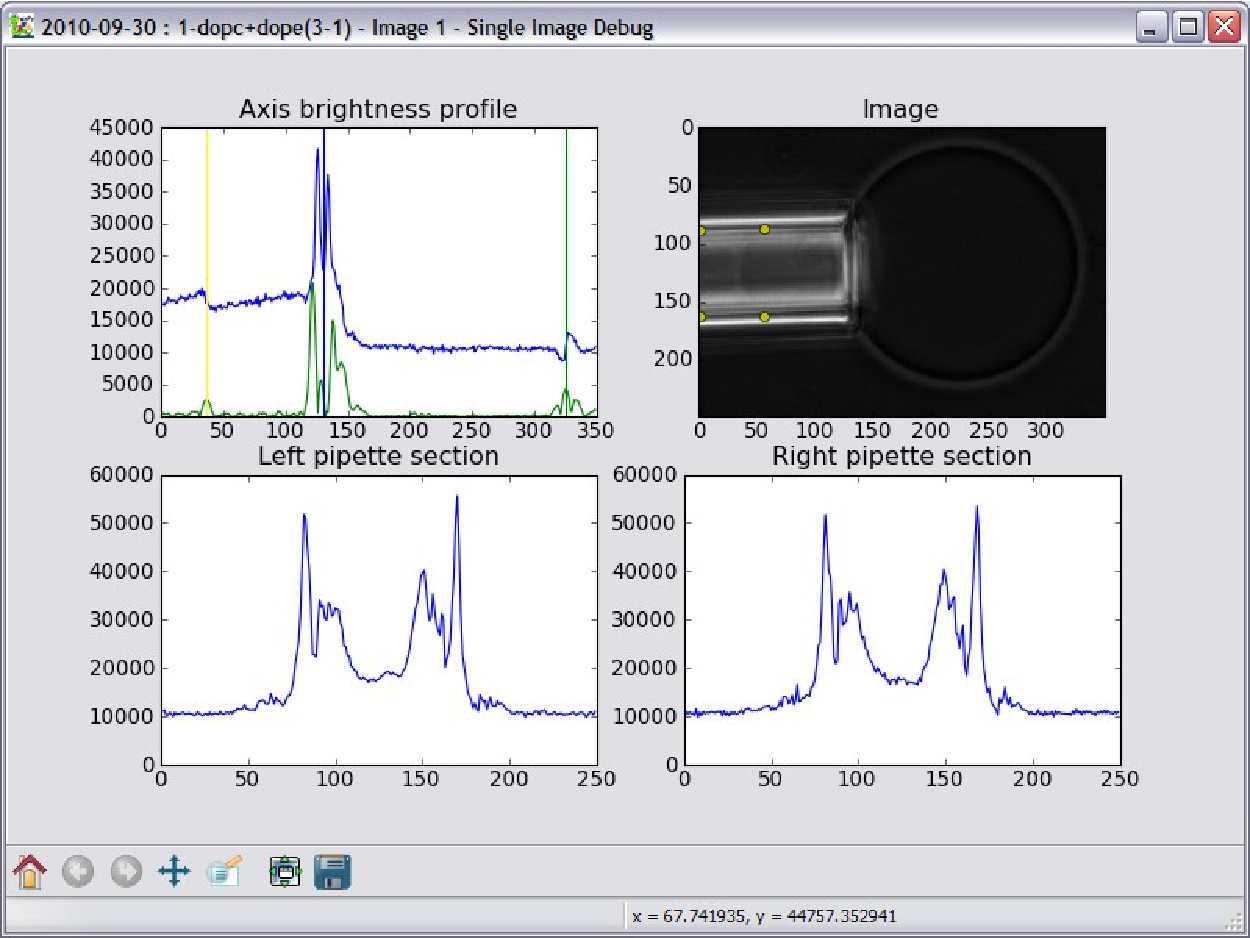
\includegraphics[width=1.00\textwidth]{figs/vampydebug.pdf}
			\caption{VAMPy single image debug window}
			\label{fig:vampydebug}
		\end{figure}
		\begin{enumerate}
			\item plot of various values for the single chose image - currently axis brightness profile and absolute value of its smoothed derivative with found features positions, found positions of pipette walls, brightness profile across pipette used to find pipette walls
			\item image toolbar - the same as on main window
			\item status bar - the same as on main window
		\end{enumerate}
\end{itemize}

\subsection{Work flow}\label{vampy-work}
\begin{enumerate}
	\item If it is the first time you run the software on this particular computer, make sure that all dependencies are installed (see \ref{vampy}).
	\item Run the program by launching file ``VamPy.pyw'' (on Windows) or from command line 'python VamPy.pyw' (Linux/Unix)
	\item Open desired folder with images to analyze (Menu$\rightarrow$File$\rightarrow$Open... or Ctrl+O or Toolbar button). You will also be prompted for file type to load (currently only PNG or TIF images are supported).
	\item If the folder contained a file ``vampy.cfg'', the program will try to load image settings (cropping, rotation) and sliders positions from it.
	\item Crop the image as desired - the smaller the image, the faster program works and less noise/artifacts it might encounter while analyzing images. You can use image slider to scroll through images and make sure that you do not crop out any significant parts. Sides of cropping are relative to original image
	\item Rotate image so that \emph{pipette sticks from the left side}. This is very important!
	\item Choose the type of image you are analyzing - phase contrast or differential contrast. For latter, choose also ``polar'' parameter, which is the side from where a ``virtual light'' is shining in your picture - if the left part is bright and the right has ``shadows'', choose ``left'' and vice versa.
	\item Check the option 'fromnames' if the pressures must be read from image filenames (as created with LabVAMP program). If not, the pressure file used for the experiment will be asked for
	\item decide for what will be counted as pipette mouth - it can be either a most bright part in the region of the pipette mouth or the most dark one ('darktip' unchecked or checked respectively) - ideally pipette tip produces a dark line, but with small pipette/bright illumination it might be blurred already beyond recognition, so you will have to define the pipette tip from the brightest pixels
	\item Adjust region, axis and pipette sliders so that on every image in the stack:
	\begin{itemize}
		\item Dashed line goes approximately along the pipette axis
		\item The darkest part of the pipette walls is always inside the estimation for pipette walls (yellow lines)
		\item The tip of the aspirated part is always to the left of the left vertical blue line
		\item The outer vesicle part crossing the pipette axis is always to the right of the right blue line
		\item The green region is as narrow as possible but always covering the pipette mouth
	\end{itemize} 
	\item You can save image settings - crop, rotation, position of sliders etc to use them next time you open these images, just press ``Save image info'' button in the toolbar. Settings will be saved as a simple tab separated ASCII-file ``vampy.cfg'' in the folder from where current images were loaded.
	\item Other parameters that affect the analysis:
	\begin{itemize}
		\item ``smoothing'' - what algorithm to use for smoothing and derivating the brightness profile
		\item ``window''- full width of the window in the smoothong filters that need it, otherwise ignored
		\item ``order''- smoothing strength, has different meaning in different filters (for example polinomial order in Savitzky-Golay, strength of blur in Gaussian)
		\item ``Extra'' - return a lot of additional info from image analysis and save them to external files (not fully implemented yet)
		\item ``Subpix'' - check to have a fitting routines for subpixel resolution (not fully implemented yet).
		\item ``Mismatch'' - determines when to discard the subpixel value for pixel value (as with subpixel resolution itself, not fully implemented yet).
	\end{itemize}
	\item Press the ``Analyse'' button. If you haven't checked ``fromnames'' check box, you will be prompted for the location of the pressure protocol file.
	\item The program automatically determines the situation when there are more than one image for each pressure and handles it correctly if all images are present, otherwise it produces an error message.
	\item In any case in the next dialog you will also be prompted for the next parameters:
	\begin{itemize}
		\item Stage number - which column in the pressure protocol file (part of the name of the image file) to use as a pressures for these images.
		\item Scale factor - conversion from pixels to micrometers, can be measured with the microscope ruler. Default value is for TELI CS-3960DCL camera and overall magnification of 20X.
		\item Pressure accuracy - needed for the calculation of tension accuracy (and thus accuracy of output parameters of fitting), determined by the accuracy of the stages moving the water vessels. Default is for PI M-535.21 linear stage.
	\end{itemize}
	\item After some processing time two windows will pop out - ``Vesicle Geometry'' and ``Dilation vs Tension''
	\item ``Vesicle Geometry'' shows you values and plots of various extracted/calculated parameters already averaged between images corresponding to the same pressure, such as measured pipette diameter, total vesicle volume, area, outer vesicle radius etc  .
	\item ``Dilation vs Tension'' window presents the corresponding plot together with its fit with one of the chosen models/algorithms, with fitted value printed on top of the plot.
	\item By using sliders you can control the region which is fitted.
	\item You can also inspect how well the image recognition worked on any particular image by choosing ``Debug$\rightarrow$Debug image'' from the menu of the main window. The Debug window will open, allowing you to check the algorithm performance.
\end{enumerate}

\subsection{Limitations}\label{vampy-limits}
Current problems/limitations/target for improvements:
\begin{itemize}
	\item Not thoroughly tested for dic-images
	\item No subpixel resolution for single images
	\item No extra data available to user
\end{itemize}